
\chapter{Add your own geographical data. Point data (with geometry)}

\pagestyle{fancy}
\fancyhf{}
\fancyhead[OC]{\leftmark}
\fancyhead[EC]{\rightmark}
%\renewcommand{\footrulewidth}{1pt}
\cfoot{\thepage}

%%%%%%%%%%%%%%%%%%%%%%%%%%%%%%%%%%%%%%%%%%%%%%%%%%%%%%%%%%%
%%%%%%%%%%%%%%%%%%%%%%%%%%%%%%%%%%%%%%%%%%%%%%%%%%%%%%%%%%%

\section{Displaying data with lots of points}

\textit{We've yet to present data of this type for a project (for modelling purposes it is more efficient to represent it as a count per LSOA), but it seems this is a very popular datatype for police, so here's an introduction. Please use the vast amount of online tutorials to find out more.}\\

Filename to use for this section: $sw\_5forces\_stop\_and\_search.csv$\\

\begin{figure}[!h]
	\centering
	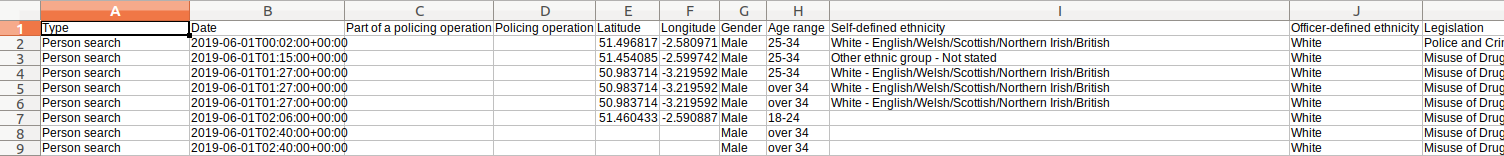
\includegraphics[width=0.6\textwidth]{images/image1.png}
	\caption{CSV file containing 38,832 stop and search instances over 3 years}
	\label{ft_fig_firstfig3}
\end{figure}

File contains our own geographical data regarding 38,832 stop and search instances over 3 years.\\
15 fields including: latitude, longitude and gender.\\
QGIS can simply take lat and long and plot point on map.\\
Tip: If get Lat and Long the wrong way round then your points will be in Africa!\\

In QGIS, opening a csv file is known as \textit{adding a delimited text layer}. There are many ways to add a delimited text layer:
\begin{enumerate}[~~~1)]
	\item
	Menu: Layer $\rightarrow$ Add Layer $\rightarrow$ Add Delimited Text Layer
	
	\item 
	\textit{Add delimited text layer} icon on a toolbar
	\begin{tabular}{@{}c@{}}
\includegraphics[width=4ex]{images/add_delimited_text_layer_icon.png}\end{tabular}
	
	\item 
	Use \textit{browse panel} to navigate to the file location
	
	\item 
	Data Source Manager icon
	\begin{tabular}{@{}c@{}}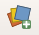
\includegraphics[width=4ex]{images/data_source_manager_icon.png}\end{tabular}
	
	
\end{enumerate}

Within the \textit{Data Source Manager / Delimited text} window, choose these settings:\\
\textbf{File name:} Navigate to the csv file: $sw\_5forces\_stop\_and\_search.csv$.\\
\textbf{Layer name} (what appears in the \textit{Layers Panel}, so choose something meaningful): stop\_search\\
\textbf{File Format}: CSV file\\
\textbf{Geometry definition} $\rightarrow$ Point coordinates $\rightarrow$  
\textbf{x field} = Longitude \& \textbf{y field} = Latitude\\
\textbf{Coordinate system}: EPSG4326 – WGS 84 (leave as default)\\

(Note: The top row of the csv file is used as the field titles.)\\

\textbf{Add}.\\
\null\newpage

\begin{figure}[!h]
	\centering
	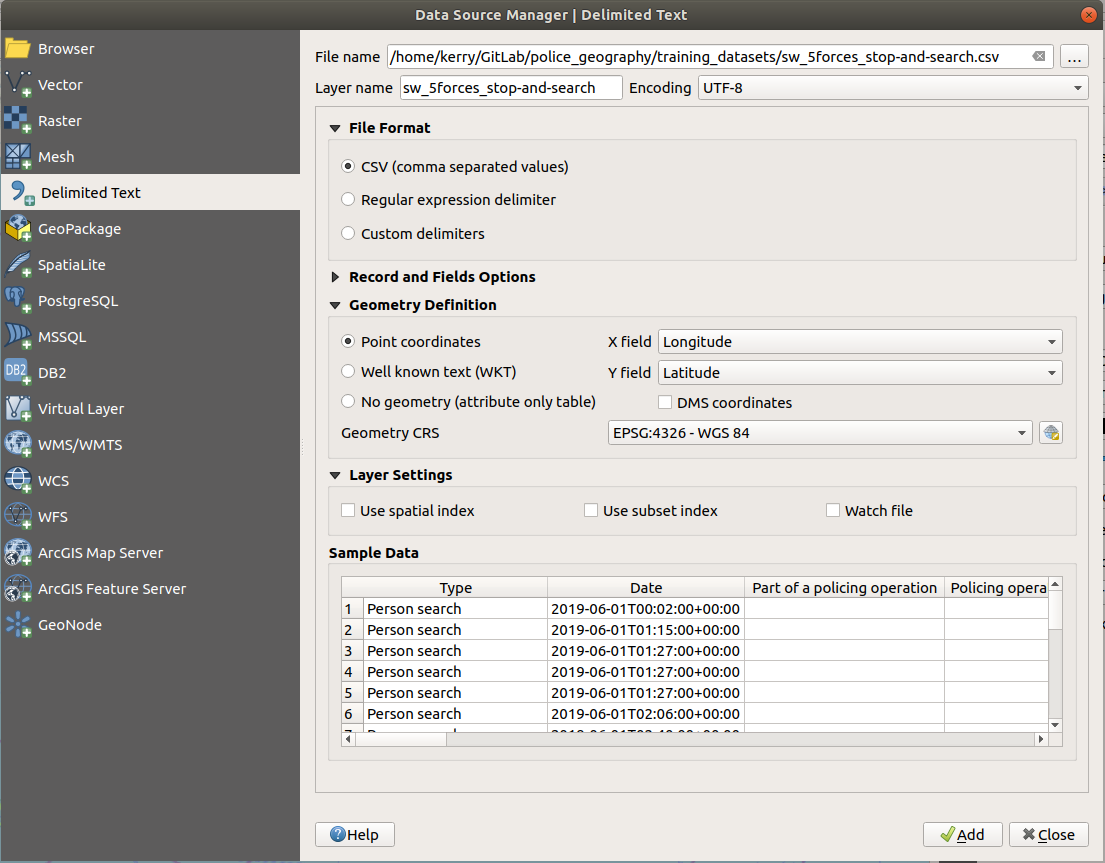
\includegraphics[width=0.6\textwidth]{images/add_delimited_text_stop_and_search.png}
	\caption{textit{Data Source Manager / Delimited text} window}
	\label{ft_fig_firstfig3}
\end{figure}
%\null\newpage

All of the 38,832 instances will will be added to your map canvas as points.\\

\begin{figure}[!h]
	\centering
	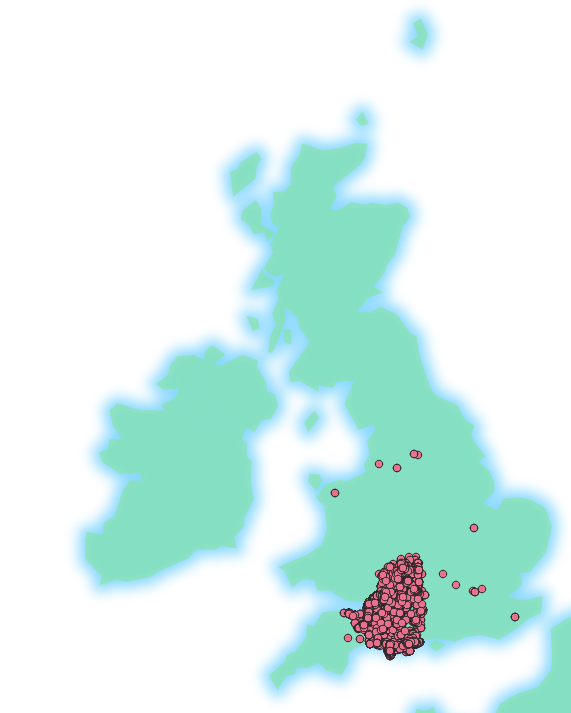
\includegraphics[width=0.4\textwidth]{images/stop_search_38832_points_over_uk.png}
	\caption{Stop and search points added to our base map}
	\label{ft_fig_firstfig3}
\end{figure}

Instantly see a benefit for plotting geographical data in a mapping software: highlights oddities. This is the dataset for the 5 SW forces. I'm curious, is there a reason why the points exist outside this region?\\

The layer name will exist in the \textit{Layers Panel}. Make sure the stop\_search layer name is above World.\\
Play with changing the order of the layers within the \textit{Layers Panel} (drag and drop).\\

\section{Attribute table}

As we saw for the World layer, each layer open in the project has an \textit{attribute table}. For this layer, each point on the map has a row of data in the layer's \textit{attribute table}.

\subsection{Open attribute table}

To open a layer's \textit{attribute table}, make sure the relative layer is highlighted in the \textit{Layers Panel}, and then click	\begin{tabular}{@{}c@{}}
\includegraphics[width=4ex]{images/attribute_table_icon.png}\end{tabular}
in the top toolbar.\\
Or right click on layer name in the \textit{Layers Panel} and select \textit{Open Attribute Table}.

\begin{figure}[!h]
	\centering
	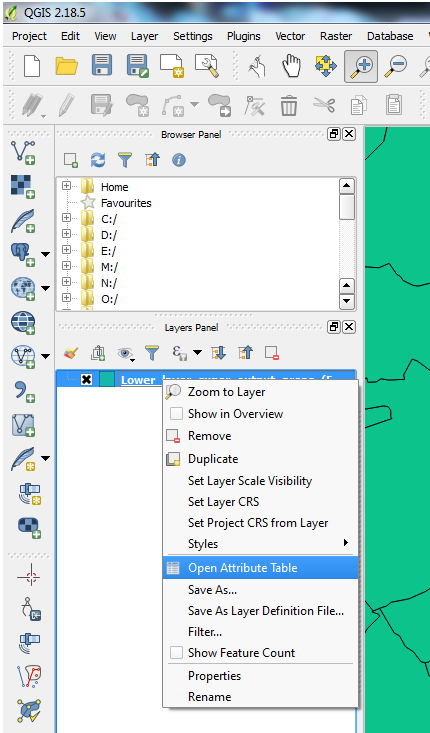
\includegraphics[width=0.3\textwidth]{images/right_click_layername.png}
	\caption{Open attribute table}
	\label{ft_fig_firstfig3}
\end{figure}

The data in the \textit{attribute table} is essentially the csv file. Can sort the data (like in excel) by clicking on the title row.\\
In GIS software, variables (columns) are referred to as \textit{fields},and rows as \textit{features}.\\

\begin{figure}[!h]
	\centering
	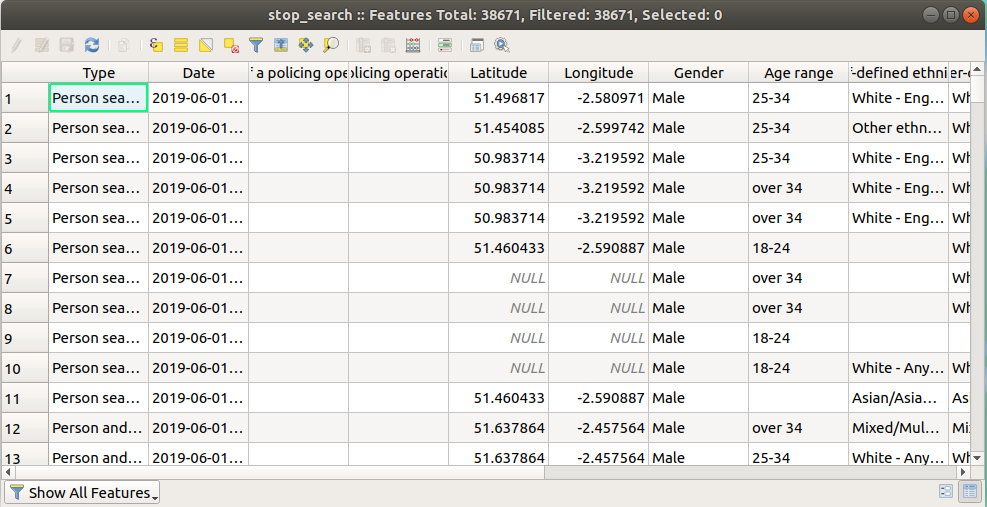
\includegraphics[width=0.6\textwidth]{images/stop_search_attribute_table.png}
	\caption{Attribute table for Stop Search layer}
	\label{ft_fig_firstfig3}
\end{figure}

\null\newpage

\subsection{Relationship between the attribute table and the map canvas}
For data with many points, it is often the case that many points will lie in the same space. So even when you have a point highlighted, it may be hidden under another point and so not visible on your map.

\subsubsection{From attribute table to map canvas}
Can select row(/s) in attribute table and see where they are in the map canvas (they become highlighted in yellow on the map - unless the point is under another point).\\

Select a row (point) in the attribute table. Notice the \textit{Attribute table} window title reports the number of total features, and any selected.\\

\begin{figure}[!h]
	\centering
	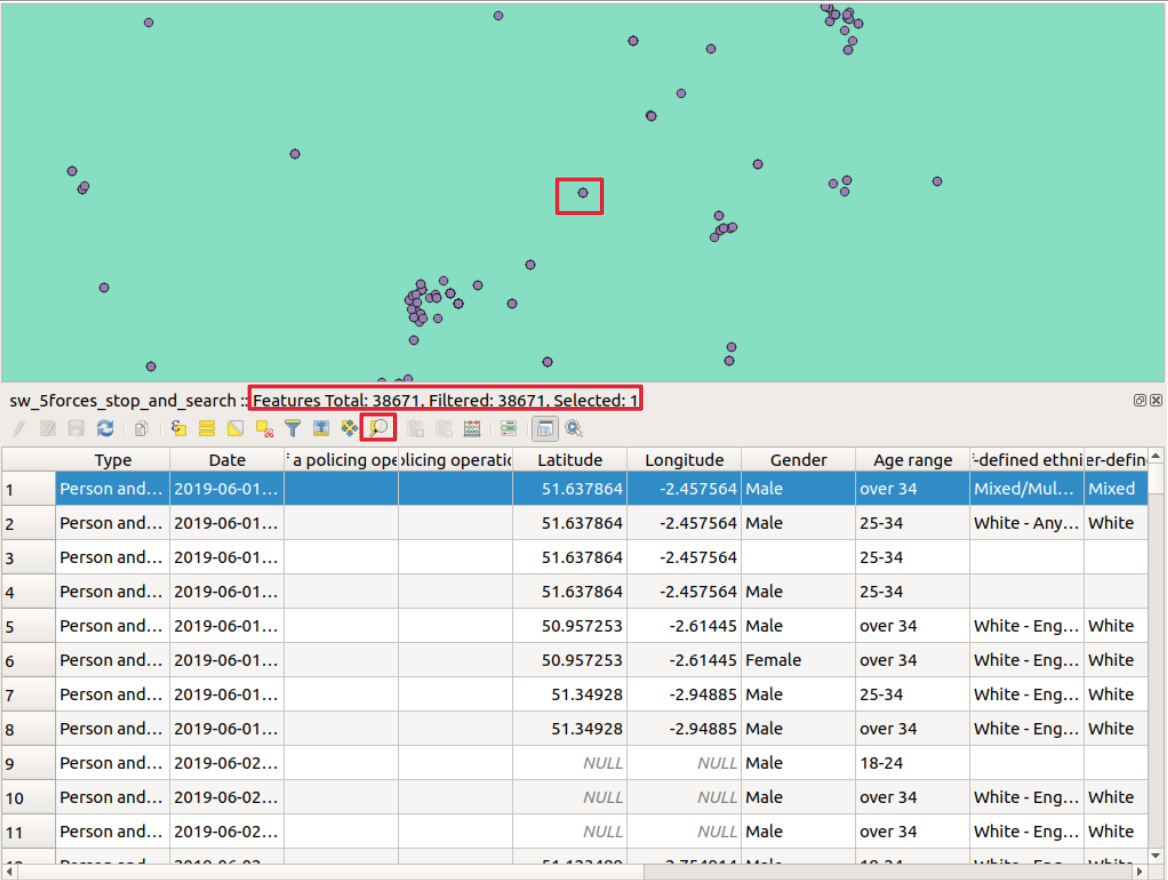
\includegraphics[width=0.5\textwidth]{images/stop_search_one_row_selected_redbox.png}%stop_search_at_tbl_select_6_features_redbx.png}%attribute_table_top_rows.png}
	\caption{Stop and search attribute table, selected 1 row with relevant point highlighted, not in yellow as it's under another point. Red boxes highlight 1) Point selected 2) Number of features selected 4) Zoom to point button}
	\label{ft_fig_firstfig3}
\end{figure}

Sometimes we can not instantly see where these features are on our map, so use the map navigation function buttons: \textit{Pan to selected} \& \textit{Zoom to selected}. These function buttons are in the Attributes \& Map Navigation toolbars, and in the Attribute Table title bar. For some cases, need to press this button a couple of times for it to take effect.

\begin{figure}[!h]
	\centering
	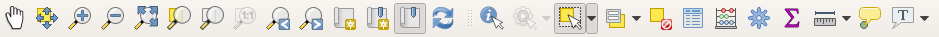
\includegraphics[width=1\textwidth]{images/attribute_and_map_navigation_toolbars_icons.png}
	\caption{Function buttons in the Attributes \& Map Navigation toolbars}
	\label{ft_fig_firstfig3}
\end{figure}

Useful to know at this stage that we can dock the attribute table to the main window, so we can see both the map canvas and the attribute table 
\begin{tabular}{@{}c@{}}
\includegraphics[width=4ex]{images/dock_attribute_table_icon.png}\end{tabular}\\

If no yellow point exists, then it will be under another point.
A useful tool to then use is Identify Feature tool. See the next section.\\
\null\newpage
To get an example which only has one point at a location (so can see the yellow selected point) sort the attribute table by the field \textit{Date}, select the top row and Zoom To Selected.
\begin{figure}[!h]
	\centering
	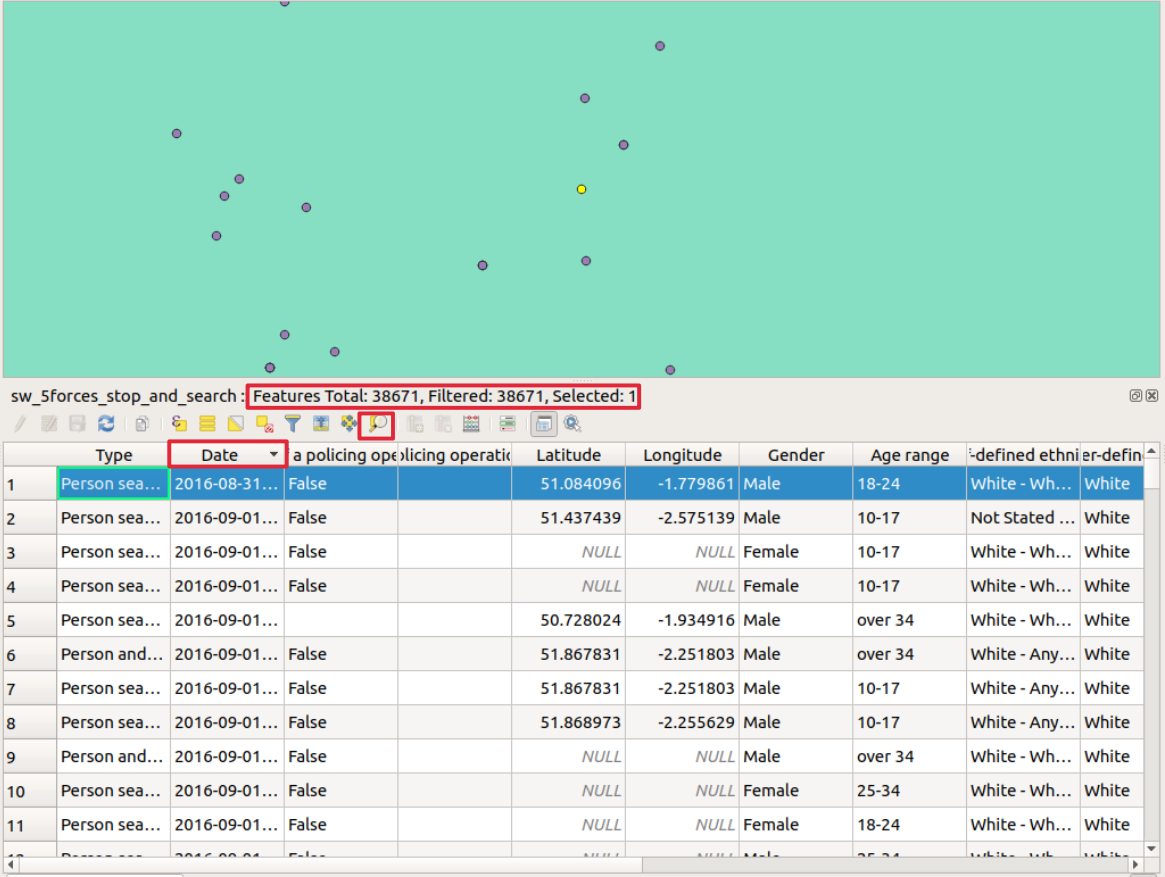
\includegraphics[width=0.5\textwidth]{images/stop_search_one_row_selected_oldest_date_redbox_docked_at_table.png}%stop_search_one_row_selected_oldest_date_redbox.png}%stop_search_at_tbl_select_6_features_redbx.png}%attribute_table_top_rows.png}
	\caption{Stop and search attribute table. Red boxes highlight 1) Order by Date 2) Selecting the oldest feature 3) Number of features selected 4) Map navigation function buttons}
	\label{ft_fig_firstfig3}
\end{figure}


\subsubsection{From map canvas to attribute table using the \textit{Identify Feature} tool}

Click the \textit{Identify Feature} icon 
\begin{tabular}{@{}c@{}}
\includegraphics[width=4ex]{images/identify_feature_icon.png}\end{tabular}

This function will only work on the top layer (as in the \textit{Layers Panel}, even if the top layer is unselected.

Click on a feature (point). Information about that feature (point) will be displayed in the \textit{Identify Results Panel}, this is essentially the values of the fields in the layer's \textit{Attribute Table}):  

\begin{figure}[!h]
	\centering
	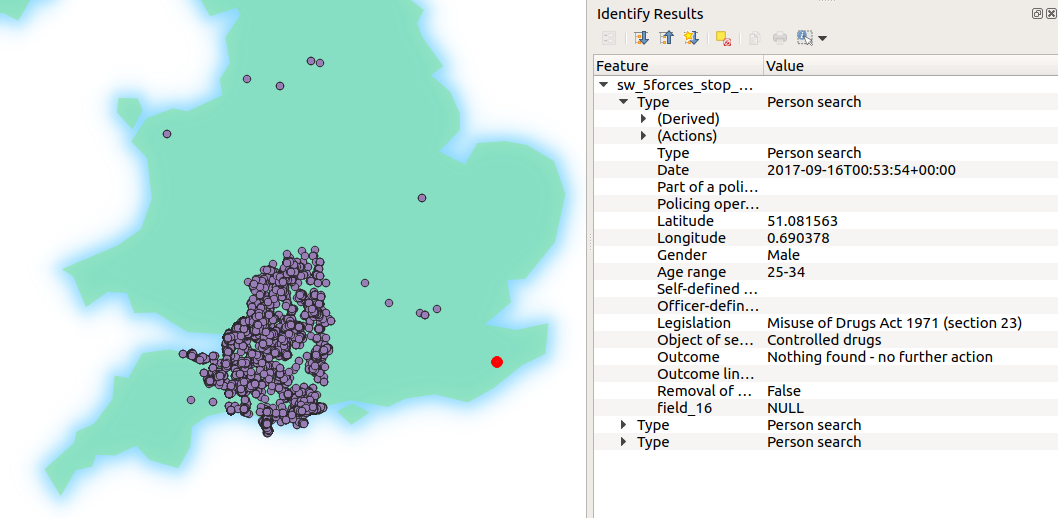
\includegraphics[width=0.55\textwidth]{images/stop_search_identify_feature.png}%identify_feature_window.png}
	\caption{}
	\label{ft_fig_firstfig3}
\end{figure}

For locations with multiple points on the same site, all of the features will appear in the \textit{Identify Results Panel}.

\subsubsection{From map canvas to attribute table using the \textit{Select Feature(s)} tool}

Alternatively, can select feature(s) (points) on the map using the \textit{Select Feature(s)} tool, the icon is in the top toolbar
\begin{tabular}{@{}c@{}}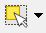
\includegraphics[width=4ex]{images/select_features_by_polygon_icon.png}\end{tabular}
, (right click to end selection).

\begin{figure}[!h]
	\centering
	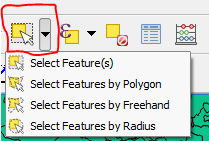
\includegraphics[width=0.2\textwidth]{images/select_features_by_polygon_dropdown.png}
	\caption{}
	\label{ft_fig_firstfig3}
\end{figure}

View the field values in the \textit{Attribute Table}, and move selection to top
\begin{tabular}{@{}c@{}}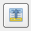
\includegraphics[width=4ex]{images/move_selection_to_top_icon.png}\end{tabular}


\begin{figure}[!h]
	\centering
	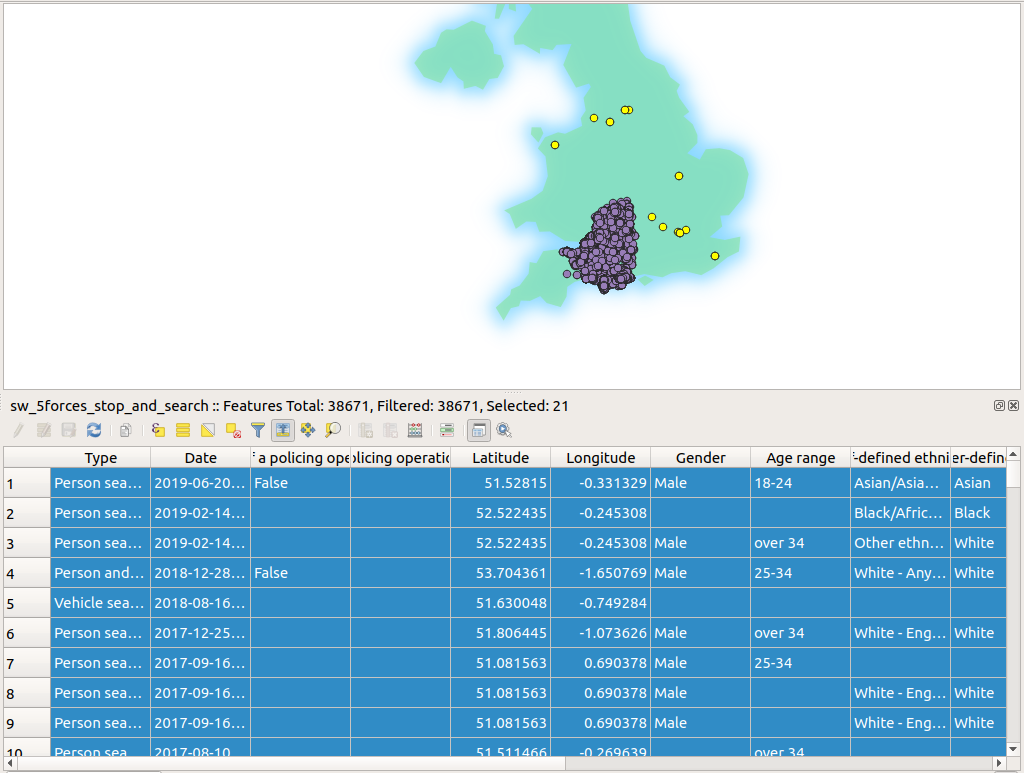
\includegraphics[width=0.55\textwidth]{images/stop_search_select_features.png}
	\caption{}
	\label{ft_fig_firstfig3}
\end{figure}
\null\newpage

Close Attribute Table (x in top right of window)\\
Close Identify Results panel.\\
Deselect all features.\\
% Not needed, done in world. INTRODUCE AND USE LAYER STYLING TO CHANGE THE SIMPLE SYMBOL.

\section{Symbology: Categorical}

We've already explored how to use the \textit{Layers Styling Panel} to change the style of a \textit{Single symbol} (to get the coastline and landmass of UK). Let's now look at how to add symbology to a layer based on a categorical field value, such as gender.\\

In the \textit{Layer Styling Panel}, select from the dropdown \textit{Categorized}\\
Column: \textit{Gender}\\
Classify.\\

If only interested in the division between Female, Male and Other, can deselect the "all other categories".

Also for each category, double click on the symbol (next to the corresponding value), select "Simple marker" to alter the size and colour of the point.

\begin{figure}[!h]
	\centering
	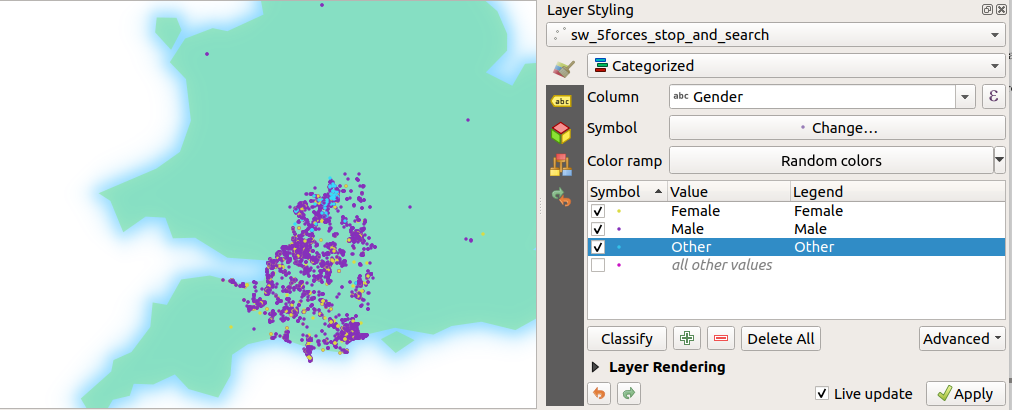
\includegraphics[width=0.5\textwidth]{images/stop_search_categorized.png}%stop_search_pt_data_gender.png}
	\caption{}
	\label{ft_fig_firstfig3}
\end{figure}

\begin{figure}[!h]
	\centering
	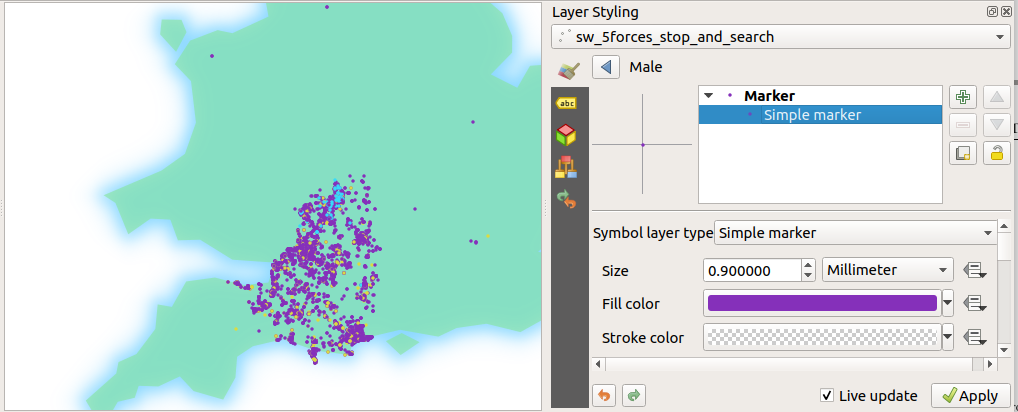
\includegraphics[width=0.5\textwidth]{images/stop_search_categorized_simple_marker.png}%stop_search_38832_points.png}
	\caption{}
	\label{ft_fig_firstfig3}
\end{figure}

Since there are too many points lying on top of each other, I would advise from interrogating your data in this manor as we already know that many points share the same location.\\

For point data that is dense, there are other options available to us.

\null\newpage
\subsection{Heatmap}
In the \textit{Layer Styling Panel}, select in the dropdown: \textit{Heatmap}.

\begin{figure}[!h]
	\centering
	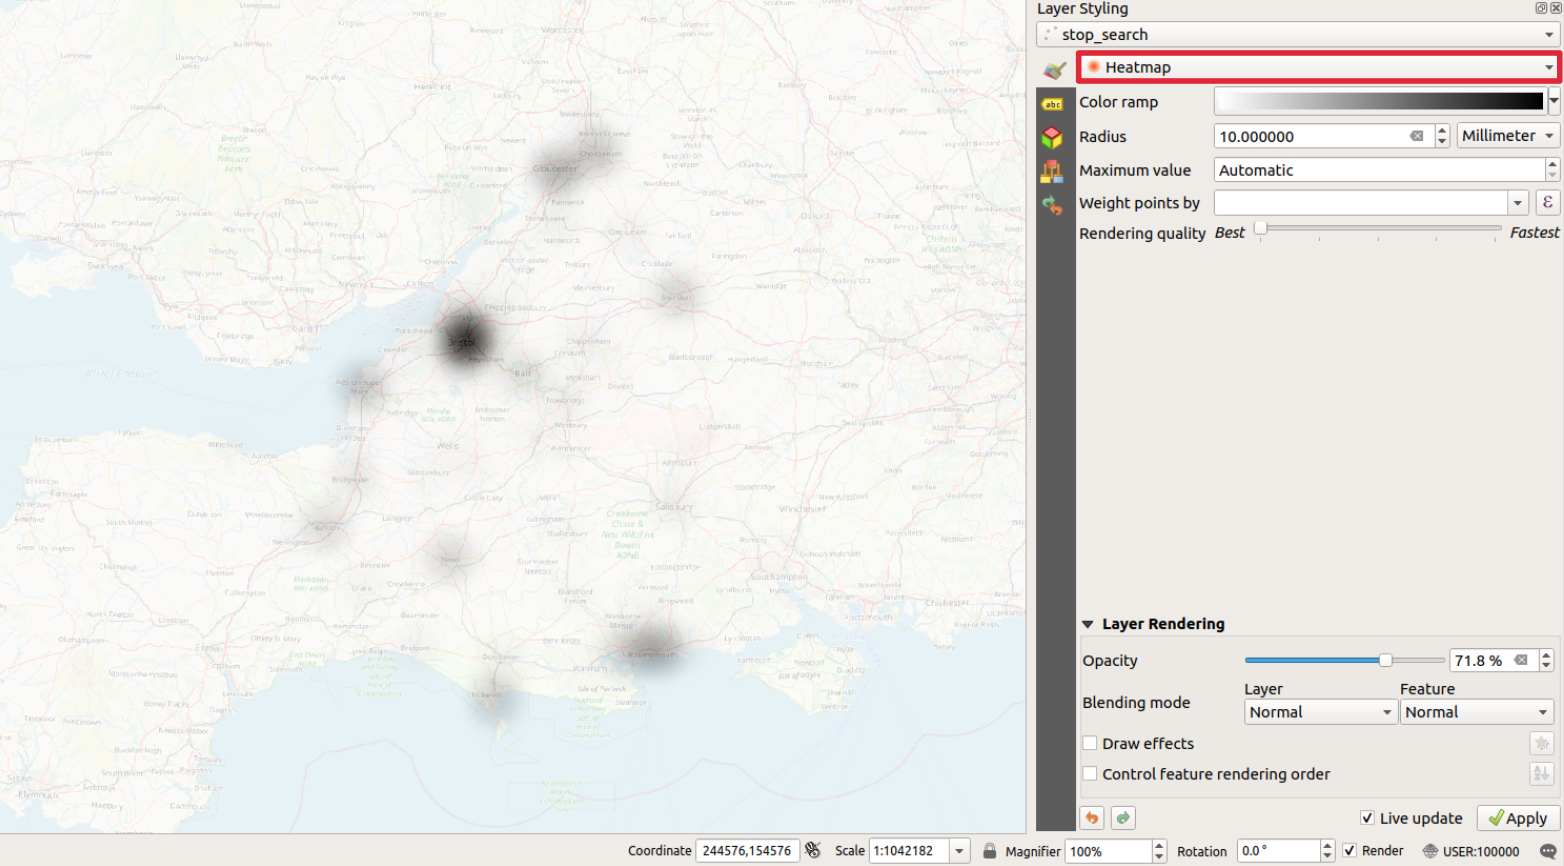
\includegraphics[width=0.5\textwidth]{images/heatmap2.png}
	\caption{}
	\label{ft_fig_firstfig3}
\end{figure}

For more information on styling heatmaps see \url{https://www.qgistutorials.com/en/docs/3/creating_heatmaps.html}, where the example data is conveniently about crimes.

\subsection{Point Cluster Renderer}

There is another option that was inspired by the maps I saw on the police website \url{https://www.police.uk/devon-and-cornwall/DEV.4055/crime/}. I wanted to see if QGIS could create something similar.\\

I found this tutorial helpful: \url{https://www.youtube.com/watch?v=-ikF1oYIpa0}\\

In the \textit{Layer Styling Panel}, select in the dropdown: \textit{Point cluster}.

\begin{figure}[!h]
	\centering
	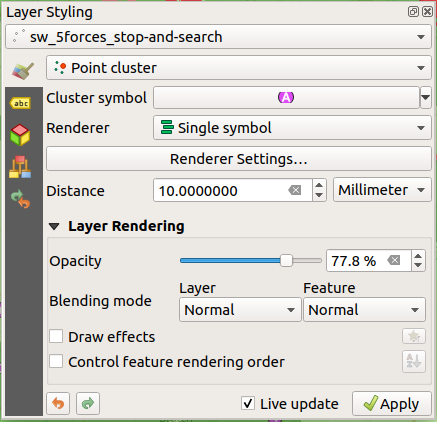
\includegraphics[width=0.5\textwidth]{images/point_cluster_layer_styling_panel.png}
	\caption{}
	\label{ft_fig_firstfig3}
\end{figure}

For the Distance units, if choose \textit{Millimetre} then the points join together based on the scale.\\
If choose \textit{Map units} then the points that join together are fixed.\\

Can also change point size depending on number:\\
Cluster symbol $\rightarrow$ Simple marker $\rightarrow$ Size $\rightarrow$ Assistant $\rightarrow$ Source: $"@cluster\_size"$\\

Change the range of "Values from" and "to".\\

\begin{figure}[!h]
	\centering
	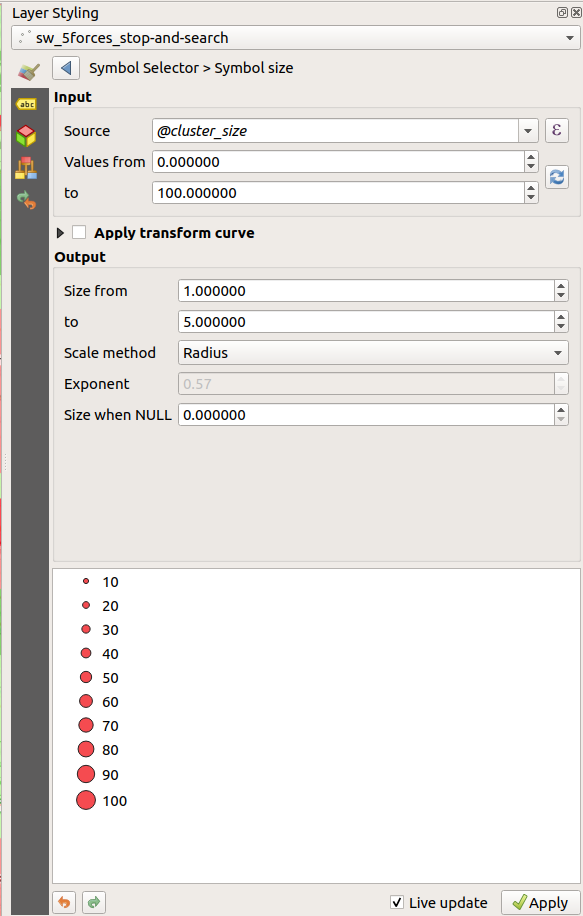
\includegraphics[width=0.5\textwidth]{images/point_clustering_cluster_size.png}
	\caption{}
	\label{ft_fig_firstfig3}
\end{figure}


\section{Displaying point data with few points}

\subsection{Add point data to map}
Filename to use for this section: $headquarters.csv$\\

This file contains our own geographical data regarding the location of the 5 police headquarters. It contains geometry data, as latitude and longitude. QGIS will use this information to plot the data on our map.\\

I created this data file from information I found online. I could only obtain postcode data for the HQ locations. QGIS can not plot postcodes. I needed to do a bit of data processing before can use this in QGIS.  Use free online databases to convert each postcode to either (1) Eastings and Northings, or (2) Latitude and longitude (as required by QGIS to display a point position)\\

\url{https://www.ordnancesurvey.co.uk/business-and-government/products/code-point-open.html}
\url{https://www.freemaptools.com/convert-uk-postcode-to-lat-lng.htm}

\begin{figure}[!h]
	\centering
	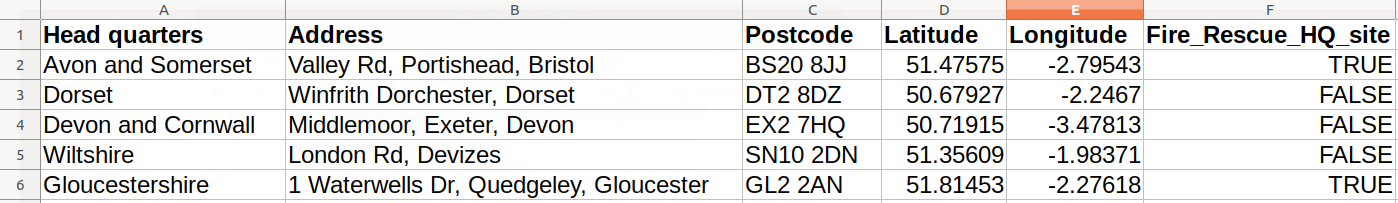
\includegraphics[width=0.8\textwidth]{images/headquarters_csv.png}
	\caption{}
	\label{ft_fig_firstfig3}
\end{figure}


Let's add this delimited file 
\begin{tabular}{@{}c@{}}
\includegraphics[width=4ex]{images/add_delimited_text_layer_icon.png}\end{tabular}
.  

Navigate to the csv file  $headquarters$.\\
Layer name (what appears in the \textit{Layers Panel}, so choose something meaningful): street\_crime\\
Select \textit{CSV file}\\
Select \textit{Geometry definition} $\rightarrow$ Point coordinates $\rightarrow$  
x field = Longitude \& y field = Latitude\\
Coordinate system (leave as default: EPSG4326 – WGS 84)\\
Top row of csv file is used as the field titles\\
Add.\\

\begin{figure}[!h]
	\centering
	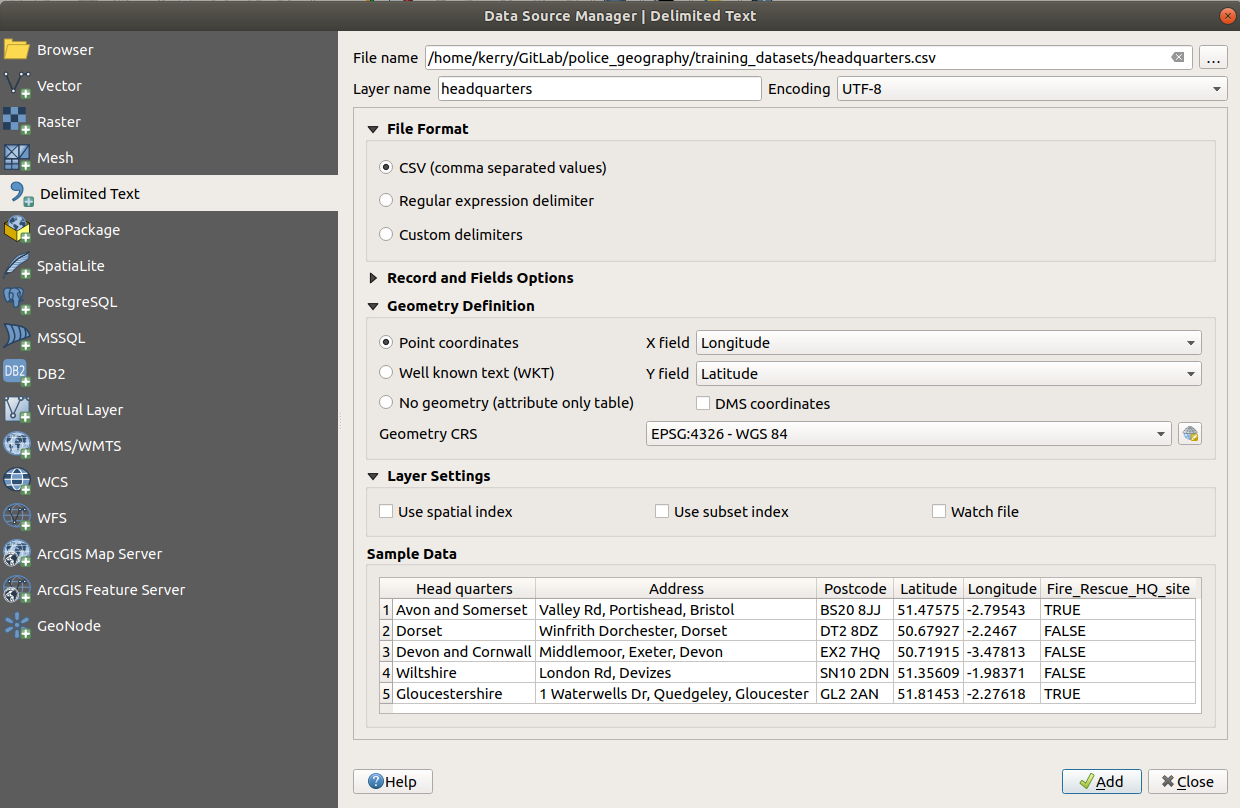
\includegraphics[width=0.8\textwidth]{images/data_source_manager_add_delimited_text.png}
	\caption{}
	\label{ft_fig_firstfig3}
\end{figure}


\textbf{TASK}. Play with the simple symbol, select a colour/shape to represent the HQs

\null\newpage

\subsection{Add categorized symbology to point data}

Like we saw for the polygons, we can also have a different symbol for our points based on a value of a field. This data has a field "Fire\_Rescue\_HQ\_site" which stores a boolean to represent whether the Police HQ location is also the site for the Fire and Rescue HQ. Let's format our points to show this information.\\

In the \textit{Layers Styling Panel}:\\
Select \textit{headquarters}\\
Select \textit{Categorized}\\
Column: Fire\_Rescue\_HQ\_site.  \\
Classify

%\begin{figure}[!h]
%	\centering
%	\%includegraphics[width=0.5\textwidth]{images/headquarters_styling1.png}
%	\caption{}
%	\label{ft_fig_firstfig3}
%\end{figure}

Choose the style for the two symbols.\\
Set legend text: Police HQ, Police \& Fire Rescue HQ


\begin{figure}[!h]
	\centering
	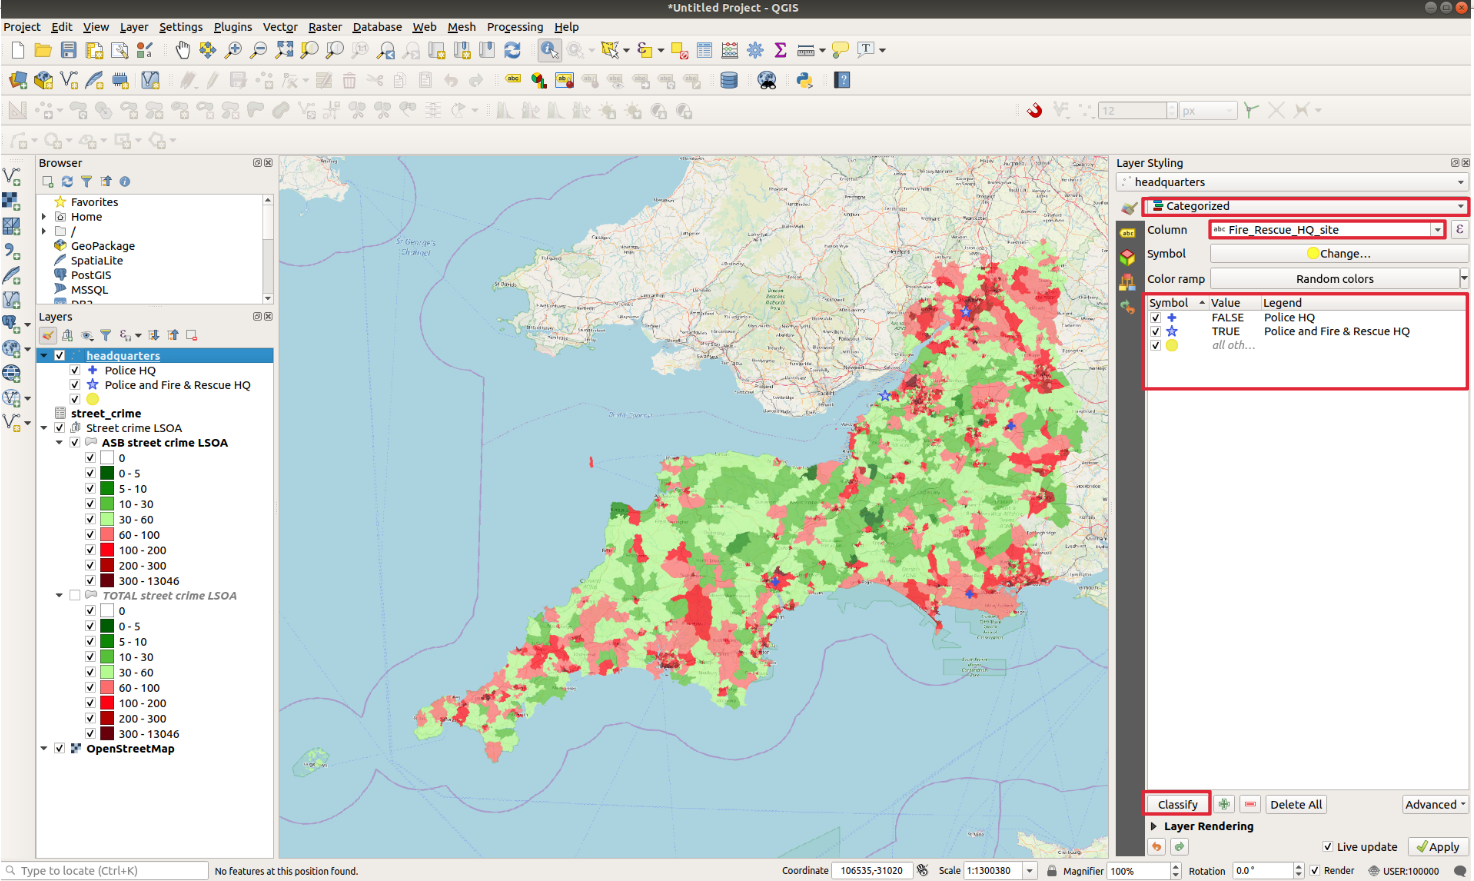
\includegraphics[width=0.7\textwidth]{images/point_data_symbology1.png}
	\caption{}
	\label{ft_fig_firstfig3}
\end{figure}

\subsection{Use rule based styles}

For more complicated allocation of a symbol to field values, can set up rules.

Can see the structure of the rules for the previous styling we chose by selecting “Rule-based” and double clicking on one of the rules.

\begin{figure}[!h]
	\centering
	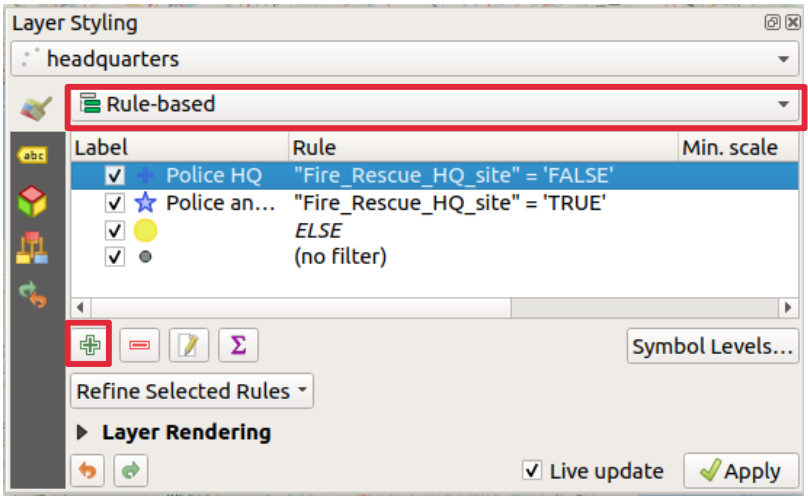
\includegraphics[width=0.5\textwidth]{images/headquarter_rule_based_styles1.png}
	\caption{}
	\label{ft_fig_firstfig3}
\end{figure}


\begin{figure}[!h]
	\centering
	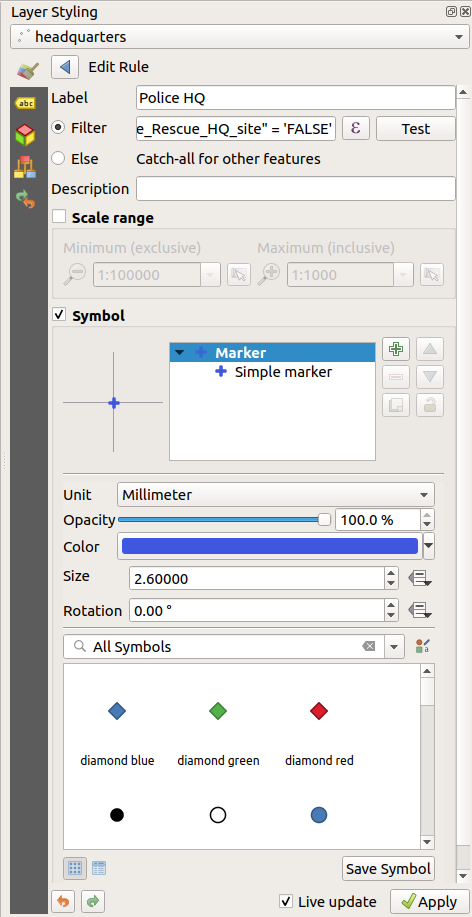
\includegraphics[width=0.3\textwidth]{images/headquarter_rule_based_styles2.png}
	\caption{}
	\label{ft_fig_firstfig3}
\end{figure}

We will set up some rule based labels later, just showing that they are possible for the symbology as well.\\

Select the green + button to add a new rule.\\

\null\newpage

